% Adjusting chapter title format for regular (numbered) chapters
\titleformat{\chapter}[display]
  {\normalfont\huge\bfseries\centering}{\chaptertitlename\ \thechapter}{20pt}{\Huge}

% Using similar styling for unnumbered chapters but without "Chapter" prefix
\titleformat{name=\chapter,numberless}
  {\normalfont\huge\bfseries\centering}{}{0pt}{\Huge}

\titlespacing*{\chapter}{0pt}{50pt}{40pt} % Adjust vertical spacing before and after the title

\chapter{Proposed Framework} % Ensures chapter numbering starts correctly
\label{chp:3}


This chapter presents a comprehensive approach for AI systems, which may consist of one or multiple DNN components, each component handle different task. My research introduces a framework that addresses each DNN separately, recognising that each has unique specifications, e.g., consider an AI system using the MNIST dataset for different purposes. One DNN might classify handwritten digits (0-9), while another might analyse pairs of digits to predict their sum or product. Although both DNNs work with digit images in this case, their properties in specifications differ due to their distinct tasks, even when using the same dataset. In other cases, such as an autonomous car, different DNNs might use different datasets designed for their specific tasks. One DNN might use labeled images for object detection (e.g., identifying pedestrians, vehicles, and road signs), while another DNN might use data on driving paths and movement for path planning to predict optimal routes. This framework provides end-to-end testing for each DNN. It consists of five components, summarized in Figure~\ref{fig:framework} and Algorithm. \ref{alg:model_robustness}

\begin{enumerate}
  \item \emph{Specification} defines key properties to guide testing. It includes details about the DNN architecture, environmental properties, testing type, and input data, like data type, sample size, and number of classes. 
    \item \emph{Sampling} involves selecting a representative subset of inputs from a potentially vast input space. Depending on the testing objectives, this subset helps ensure that the tests are meaningful and cover various scenarios effectively.
    \item \emph{Testcase Generation} applies the properties mentioned in the specifications to the sampled data to generate test cases.
    \item \emph{Testing Graph Analysis} conducts both local and global coverage assessments. Locally, it focuses on an individual property to check its correctness. Globally, it examines multiple properties to understand their interdependencies and overall system behavior. By modeling these dependencies probabilistically, testing graph analysis provides a comprehensive view of AI system.
    \item \emph{Error Summarisation} quantify the performance of the AI system by compiling and analyzing recorded errors. This analysis generates graphical reports and recommendations, helping to refine and improve the models.
\end{enumerate}

\begin{figure*}
  \centering
  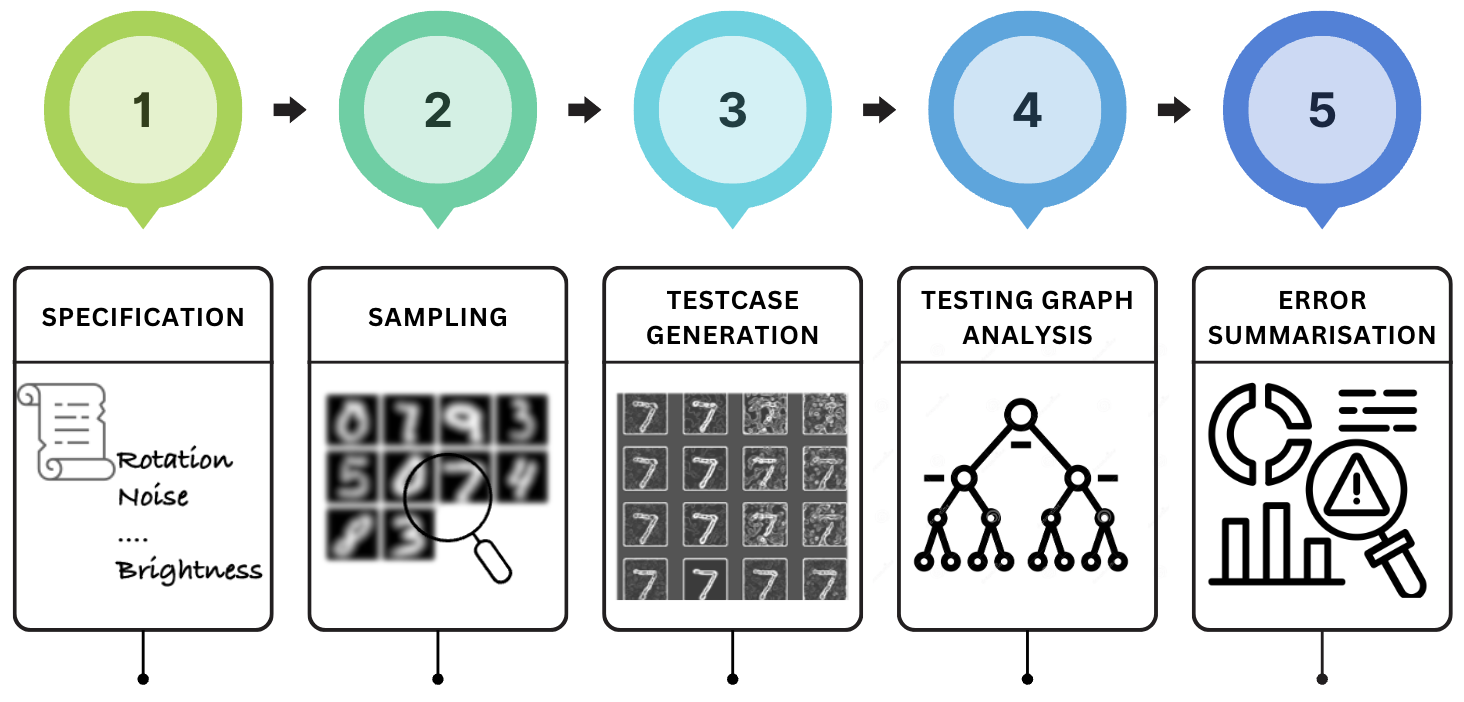
\includegraphics[width=\linewidth]{figures/fivesteps.png}
  \caption{Overview of the Proposed Framework}
  \label{fig:framework}
\end{figure*}

My research focus on AI systems with DNN components performing various tasks, which may include classification, regression, clustering and more. Each DNN within the system has unique specifications. Formally, we define an AI system $ \mathcal{S} $ as follows:

$\mathcal{F}$ is the functional unit comprises $n$ DNN components $ f_1, \dots, f_n $, each handling different tasks, and a symbolic (software) component $ \omega $ that integrates the outputs of these DNNs. Given an input $\vec{x} = (x_1, \dots, x_n)$, where each $x_i$ represents an input from the respective dataset of $f_i$, the output $\mathcal{F}(\vec{x})$ is defined as $\omega(f_1(x_1), \dots, f_n(x_n))$. Each DNN component $f_i$ processes its input $x_i$ according to its specific dataset.


\section{Specification}
The first component of this framework is formalized to specify model architecture $\mathcal{M}$, properties, testing type, and input data characteristics $\mathcal{D}$. 

The specifications $\mathcal{S}_{\text{specs}}$ include all classes (classification task) by default, but users can adjust this to test specific classes based on their needs.

It is essential to specify the type of testing $\mathcal{T}$ within the $\mathcal{S}_{\text{specs}}$, as different methods are employed based on this choice. In black-box testing $\mathcal{T}_{\text{black}}$, semantic adversarial properties $\mathcal{P}_{\text{sem}}$ are applied by adjusting the input data $\mathcal{D}$ without any knowledge of the model's internal details. In white-box testing $\mathcal{T}_{\text{white}}$, adversarial attacks $\mathcal{P}_{\text{adv}}$ are used by accessing the model's internal structure and parameters. Grey-box testing $\mathcal{T}_{\text{grey}}$ combines aspects of both, utilizing partial knowledge of the model’s structure to inform the testing process. 



\begin{example}
  \label{ex:mnist-adder-specification}
  Consider the AI system $\mathcal{S}_{\text{adder}}$, an \emph{MNIST Digit Adder}, which is specified as $\mathcal{S}_{\text{adder}} = (\mathcal{F}, \mathcal{D})$. In this system, the functional unit $\mathcal{F}$ consists of a DNN component $\mathcal{M}_{\text{CNN}}$, which is a Convolutional Neural Network (CNN) designed to recognize digits ranging from 0 to 9. The dataset $\mathcal{D}$ provides input in the form of images, and a software component $\omega$ is used to perform the addition of the recognized digits. 

  Formally, we define $\mathcal{F} = (\{\mathcal{M}_{\text{CNN}}\}, \omega)$, where $\omega$ integrates the output of the DNN. The function $\mathcal{M}_{\text{CNN}}$ takes single digit as an input and recognizes the digits. The software component $\omega$ can then pick any two recognized digits and compute their sum. For example, $\mathcal{S}_{\text{adder}}$ can perform the task of digit addition:
  \begin{equation}
    \mathcal{S}_{\text{adder}}(x_1, x_2) = \omega(\mathcal{M}_{\text{CNN}}(x_1), \mathcal{M}_{\text{CNN}}(x_2)),
  \end{equation}
  where $\omega(a, b) = a + b$. Given two digits $x_1$ and $x_2$, $\mathcal{S}_{\text{adder}}$ recognizes the digits and computes their sum.

  The specifications $\mathcal{S}_{\text{specs}}$ for this system include the following key elements: The DNN component $\mathcal{M}_{\text{CNN}}$ is a pre-trained CNN with a typical architecture involving a convolutional layer (32 filters, kernel size 3x3, ReLU activation), followed by a max pooling layer (2x2), a flattened layer, a fully connected layer with 128 neurons (ReLU), and an output layer with 10 neurons using softmax activation. The input data $\mathcal{D}$ consists of 10,000 test samples of digits, each labeled with one of 10 classes representing the digits 0 to 9. 

  $\mathcal{S}_{\text{adder}}$ is evaluated using both black-box and white-box testing methods. In black-box testing $\mathcal{T}_{\text{black}}$, semantic adversarial properties such as rotation, brightness adjustment, blur, shear, and contrast modification are applied to the input data without accessing the internal structure of $\mathcal{M}_{\text{CNN}}$. Specifically, $\mathcal{S}_{\text{adder}}$ robustness is tested against rotations within a range of 3 to 30 degrees and brightness adjustments between 0.5 and 1.5. In white-box testing $\mathcal{T}_{\text{white}}$, adversarial examples are generated by utilizing the internal structure and parameters of $\mathcal{M}_{\text{CNN}}$, like Fast Gradient Sign Method (FGSM), Projected Gradient Descent (PGD), AdamPGD, and Deepfool.
\end{example}


\textbf{Note:} Grey-box testing, involving partial model access, will be explored in future work.
\section{Sampling}
The sampling process is designed to identify both efficient and corner cases, focusing on hard-to-learn examples to enhance the robustness of the model. Data is sampled according to the requirements specified in the specifications. By default, all classes are tested, but users can customize the classes to be sampled based on specific requirements. The sampling approach is applied as follows for each classifier $f_i$ independently:

The full sample $\mathcal{X}_i$ for classifier $f_i$, $i=1,\dots,n$, is computed by applying the sampling method directly to the dataset $\mathcal{D}_i$:

\begin{equation}
\mathcal{X}_i = \text{Sampling}(\mathcal{D}_i)
\end{equation}

Here, $\mathcal{D}_i$ represents the dataset associated with each classifier $f_i$. In cases where all classifiers share the same dataset, $\mathcal{D}_i$ may be identical across all $i$, denoted simply as $\mathcal{D}$. However, if the datasets differ for each classifier, they are represented individually as $\mathcal{D}_1, \mathcal{D}_2, \dots, \mathcal{D}_n$ to reflect the specific dataset for each $f_i$.



This sampling method is designed to balance the dataset and ensure that both typical and challenging cases are adequately represented, thereby improving the evaluation of the model's performance across a variety of scenarios.


\begin{example}
  \label{ex:sampling}
  To further illustrate the sampling process, consider the classifier $\mathcal{M}_{\text{CNN}}$ and $\mathcal{D}$ from Example~\ref{ex:mnist-adder-specification}. For each class $c$ in $\mathcal{D}$, we begin with the samples specified in specification, forming the initial subset $\mathcal{X}_{\text{mnist}}$. This subset is then enhanced by applying a hybrid sampling method, that combines Borderline-SMOTE focuses on creating samples near decision boundaries, while ADASYN targets hard-to-learn examples, ensuring that both typical and challenging cases are effectively covered. The final sample $\mathcal{X}_{\text{hyb}}$ for testing is obtained as:
  

  \begin{equation}
    \mathcal{X}_{\text{hyb}} = \text{HybridSampling}(\mathcal{X}_{\text{mnist}})
  \end{equation}

  where $\mathcal{X}_{\text{hyb}}$ is new sampled data. HybridSampling method combines Borderline-SMOTE and ADASYN. This process ensures a balanced and comprehensive set of test samples, covering both typical and challenging cases for robust evaluation of $\mathcal{M}_{\text{CNN}}$.
\end{example}




\begin{tcolorbox}[colback=purple!2!white, colframe=purple, title=Challenges in Sampling]
  \begin{itemize}
    \item \textbf{Synthetic Sample Quality:} Ensuring generated samples represent true corner cases, not noise.
    \item \textbf{Computational Overhead:} Managing the intensive computation required for hybrid sampling.
 
  \end{itemize}

\end{tcolorbox}


\section{Test Case Generation}

The test case generation process is designed to create a comprehensive set of test cases that evaluate the robustness of the AI system, as outlined in the specifications. Test cases are generated by applying specified perturbations to the resampled data, ensuring that the system is rigorously evaluated under various conditions.

For each classifier $f_i$, $i = 1, \dots, n$, test cases are generated based on the perturbations defined in the specifications. The test cases $\mathcal{T}_i$ for classifier $f_i$ are generated as follows:

\begin{equation}
\mathcal{T}_i = \text{GenerateTestCases}(\mathcal{X}_i, \mathcal{P}_i)
\end{equation}

Here, $\mathcal{X}_i$ represents the sampled data for classifier $f_i$, and $\mathcal{P}_i$ denotes the set of perturbations to be applied. The method $\text{GenerateTestCases}$ applies these perturbations to create the test cases, which are then used to assess the model's performance.

\begin{example}
  \label{ex:test-case-generation-math}
   $\mathcal{S}_{\text{adder}}$ evaluated using both black-box and white-box testing methods as specified in Example~\ref{ex:mnist-adder-specification}. The test cases are generated by applying various perturbations to the resampled data $\mathcal{X}_{\text{hyb}}$ for classifier $\mathcal{M}_{\text{CNN}}$ mentioned in Example~\ref{ex:mnist-adder-specification}.

  For black-box testing, let $\mathcal{P}_{\text{black}} = \{\text{Rotation}, \text{Brightness}, \text{Blur}, \text{Shear}, \text{Contrast}\}$ represent the set of semantic adversarial properties applied without accessing the internal structure of $\mathcal{M}_{\text{CNN}}$. The test cases generated for black-box testing are:
  
  \begin{equation}
  \mathcal{T}_{\text{black},i} = \bigcup_{p \in \mathcal{P}_{\text{black}}} \text{ApplyPerturbation}(p, \mathcal{X}_{\text{hyb}})
  \end{equation}
  
  For white-box testing, where the internal structure of $\mathcal{M}_{\text{CNN}}$ is utilized, let $\mathcal{P}_{\text{white}} = \{\text{FGSM}, \text{PGD}, \text{AdamPGD}, \text{Deepfool}\}$ represent the set of adversarial attack methods. The test cases generated for white-box testing are:
  \begin{equation}
  \mathcal{T}_{\text{white},i} = \bigcup_{a \in \mathcal{P}_{\text{white}}} \text{GenerateAdversarial}(a,\mathcal{X}_{\text{hyb}}, \mathcal{M}_{\text{CNN}})
  \end{equation}

  The overall set of test cases $\mathcal{T}_i$ for classifier $f_i$ is the union of the black-box and white-box test cases:
  \begin{equation}
  \mathcal{T}_i = \mathcal{T}_{\text{black},i} \cup \mathcal{T}_{\text{white},i}
  \end{equation}
\end{example}


\section{Testing Graph Analysis}

This component helps to evaluate the coverage of the AI system under various properties given in specification. This analysis is conducted into two main aspects: \emph{Local Coverage} and \emph{Global Coverage}.

\subsection{Local Coverage}

Local coverage evaluates the correctness of the system for each individual class. For each class $c$ the local coverage is assessed by passing testcases to the system and check its correctness. The system is then tested with these perturbed samples to check if it predicts the correct class. If the system fails to predict correctly, this indicates the presence of counterexamples for that specific class.

The local coverage for a class $c$ under perturbation $p$ is defined as:

\[
\text{Local Coverage}(c, p) = \frac{1}{|\mathcal{X}_i^c|} \sum_{x \in \mathcal{X}_i^c} \mathbb{I}[f_i(p(x)) = c]
\]

where:
\begin{itemize}
  \item $\mathbb{I}[f_i(p(x)) = c]$ is an indicator function that equals 1 if the classifier $f_i$ correctly predicts class $c$ for the perturbed input $p(x)$, and 0 otherwise.
  \item $|\mathcal{X}_i^c|$ represents the number of samples in class $c$.
\end{itemize}


\begin{example}
  \label{ex:local-robustness}
  Consider the class $c = 3 $ and the perturbation $p $ being a rotation by 25 degrees. For a set of three images $x_1, x_2, x_3 $ from class $c $, suppose the classifier correctly predicts the class for $x_1$ and $x_2$ but misclassifies $x_3$. The local robustness for this rotation perturbation is calculated as:

\[
  \text{Local Coverage}(3, \text{rotation}) = \frac{1}{3} \left( \mathbb{I}[f_i(\text{rotate}(x_1, 25^\circ)) = 3] + \mathbb{I}[f_i(\text{rotate}(x_2, 25^\circ)) = 3] \right.
\]
\[
  \left. + \mathbb{I}[f_i(\text{rotate}(x_3, 25^\circ)) = 3] \right)
\]


  If the indicator values are 1, 1, and 0 respectively, the local robustness would be:

  \begin{equation}
  \text{Local Coverage}(3, \text{rotation}) = \frac{2}{3} \approx 0.67
\end{equation}

\end{example}
\begin{figure*}[h]
  \centering
  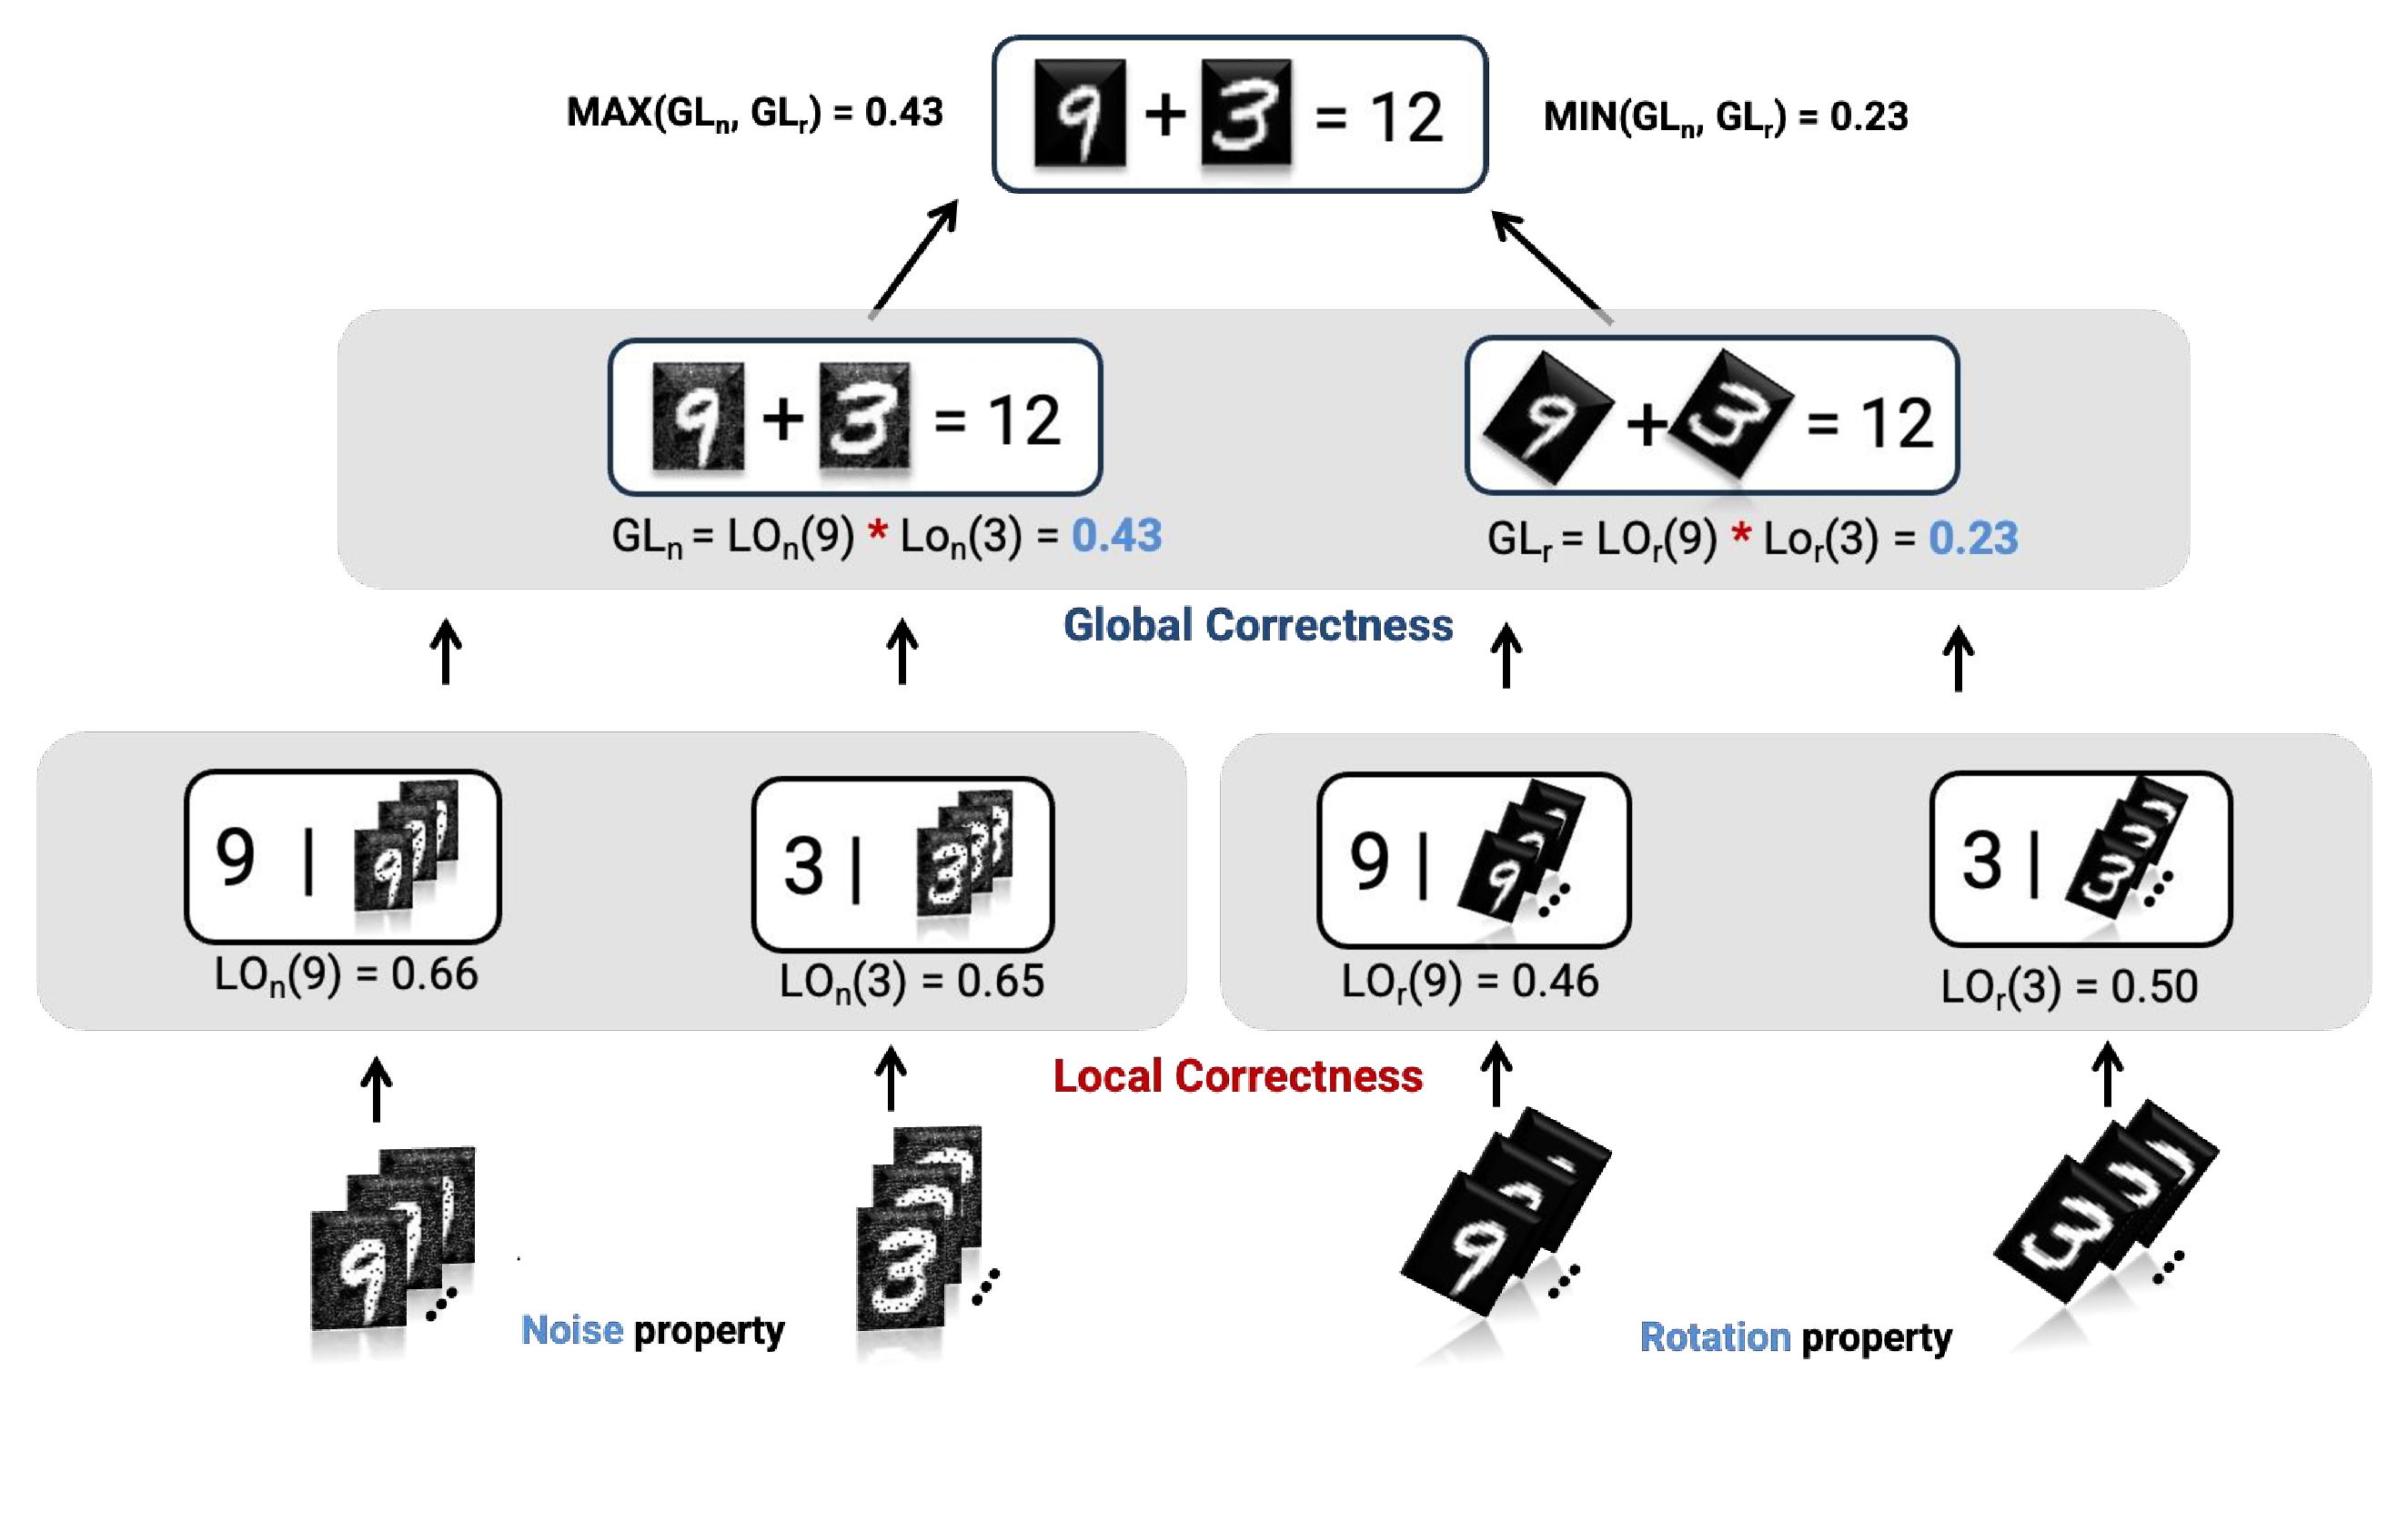
\includegraphics[width=\textwidth]{figures/noise_rotation_localcal_global.pdf}
  \caption{Global Coverage}
  \label{global}
\end{figure*}

\subsection{Global Coverage}

Global coverage evaluates the correctness across multiple classes and perturbations. It provides an aggregate measure of how well AI system performs under various properties as shown in Figure. \ref {global}.

For a given set of perturbations \( \mathcal{P} \) and class \( c \), global coverage is defined as:

\begin{equation}
\text{Global Coverage}(c, \mathcal{P}) = \frac{1}{|\mathcal{P}|} \sum_{p \in \mathcal{P}} \text{Local Coverage}(c, p)
\end{equation}

Additionally, global coverage can be evaluated for combined properties using logical relationships (AND/OR) between them:

\textbf{AND Relationship:} 
\begin{equation}
\text{Global Coverage}_{\text{AND}} = \prod_{p \in \mathcal{P}} \text{Local Coverage}(c, p)
\end{equation}

\textbf{OR Relationship:}
\begin{equation}
\text{Global Coverage}_{\text{OR}} = \sum_{p \in \mathcal{P}} \text{Local Coverage}(c, p) - \prod_{p \in \mathcal{P}} \text{Local Coverage}(c, p)
\end{equation}

\begin{example}
Consider a pair of images \( (x_1, x_2) \) representing the digits '3' and '5'. Let the transformation \( T \) be rotation. If the model's confidence scores for these transformations are as follows:

\begin{equation}
\begin{aligned}
&f_i(\text{rotation}(x_1)) = 0.78, \\
&f_i(\text{rotation}(x_2)) = 0.85,
\end{aligned}
\end{equation}

For the AND relationship, the global robustness for the pair is computed as follows:

\begin{equation}
\text{Global Robustness}_{\text{AND}} = 0.78 \times 0.85 \approx 0.663
\end{equation}

For the OR relationship, the global coverage for the pair is computed as follows:

\begin{equation}
\text{Global Robustness}_{\text{OR}} = 0.78 + 0.85 - (0.78 \times 0.85) \approx 0.967
\end{equation}

These probabilities are calculated by Problog.

\end{example}


\section{Error Summarization}

Error summarization involves evaluating the performance of the AI system by quantifying errors as shown in Figure~\ref{Summarization}.

\begin{figure*}[h]
    \centering
    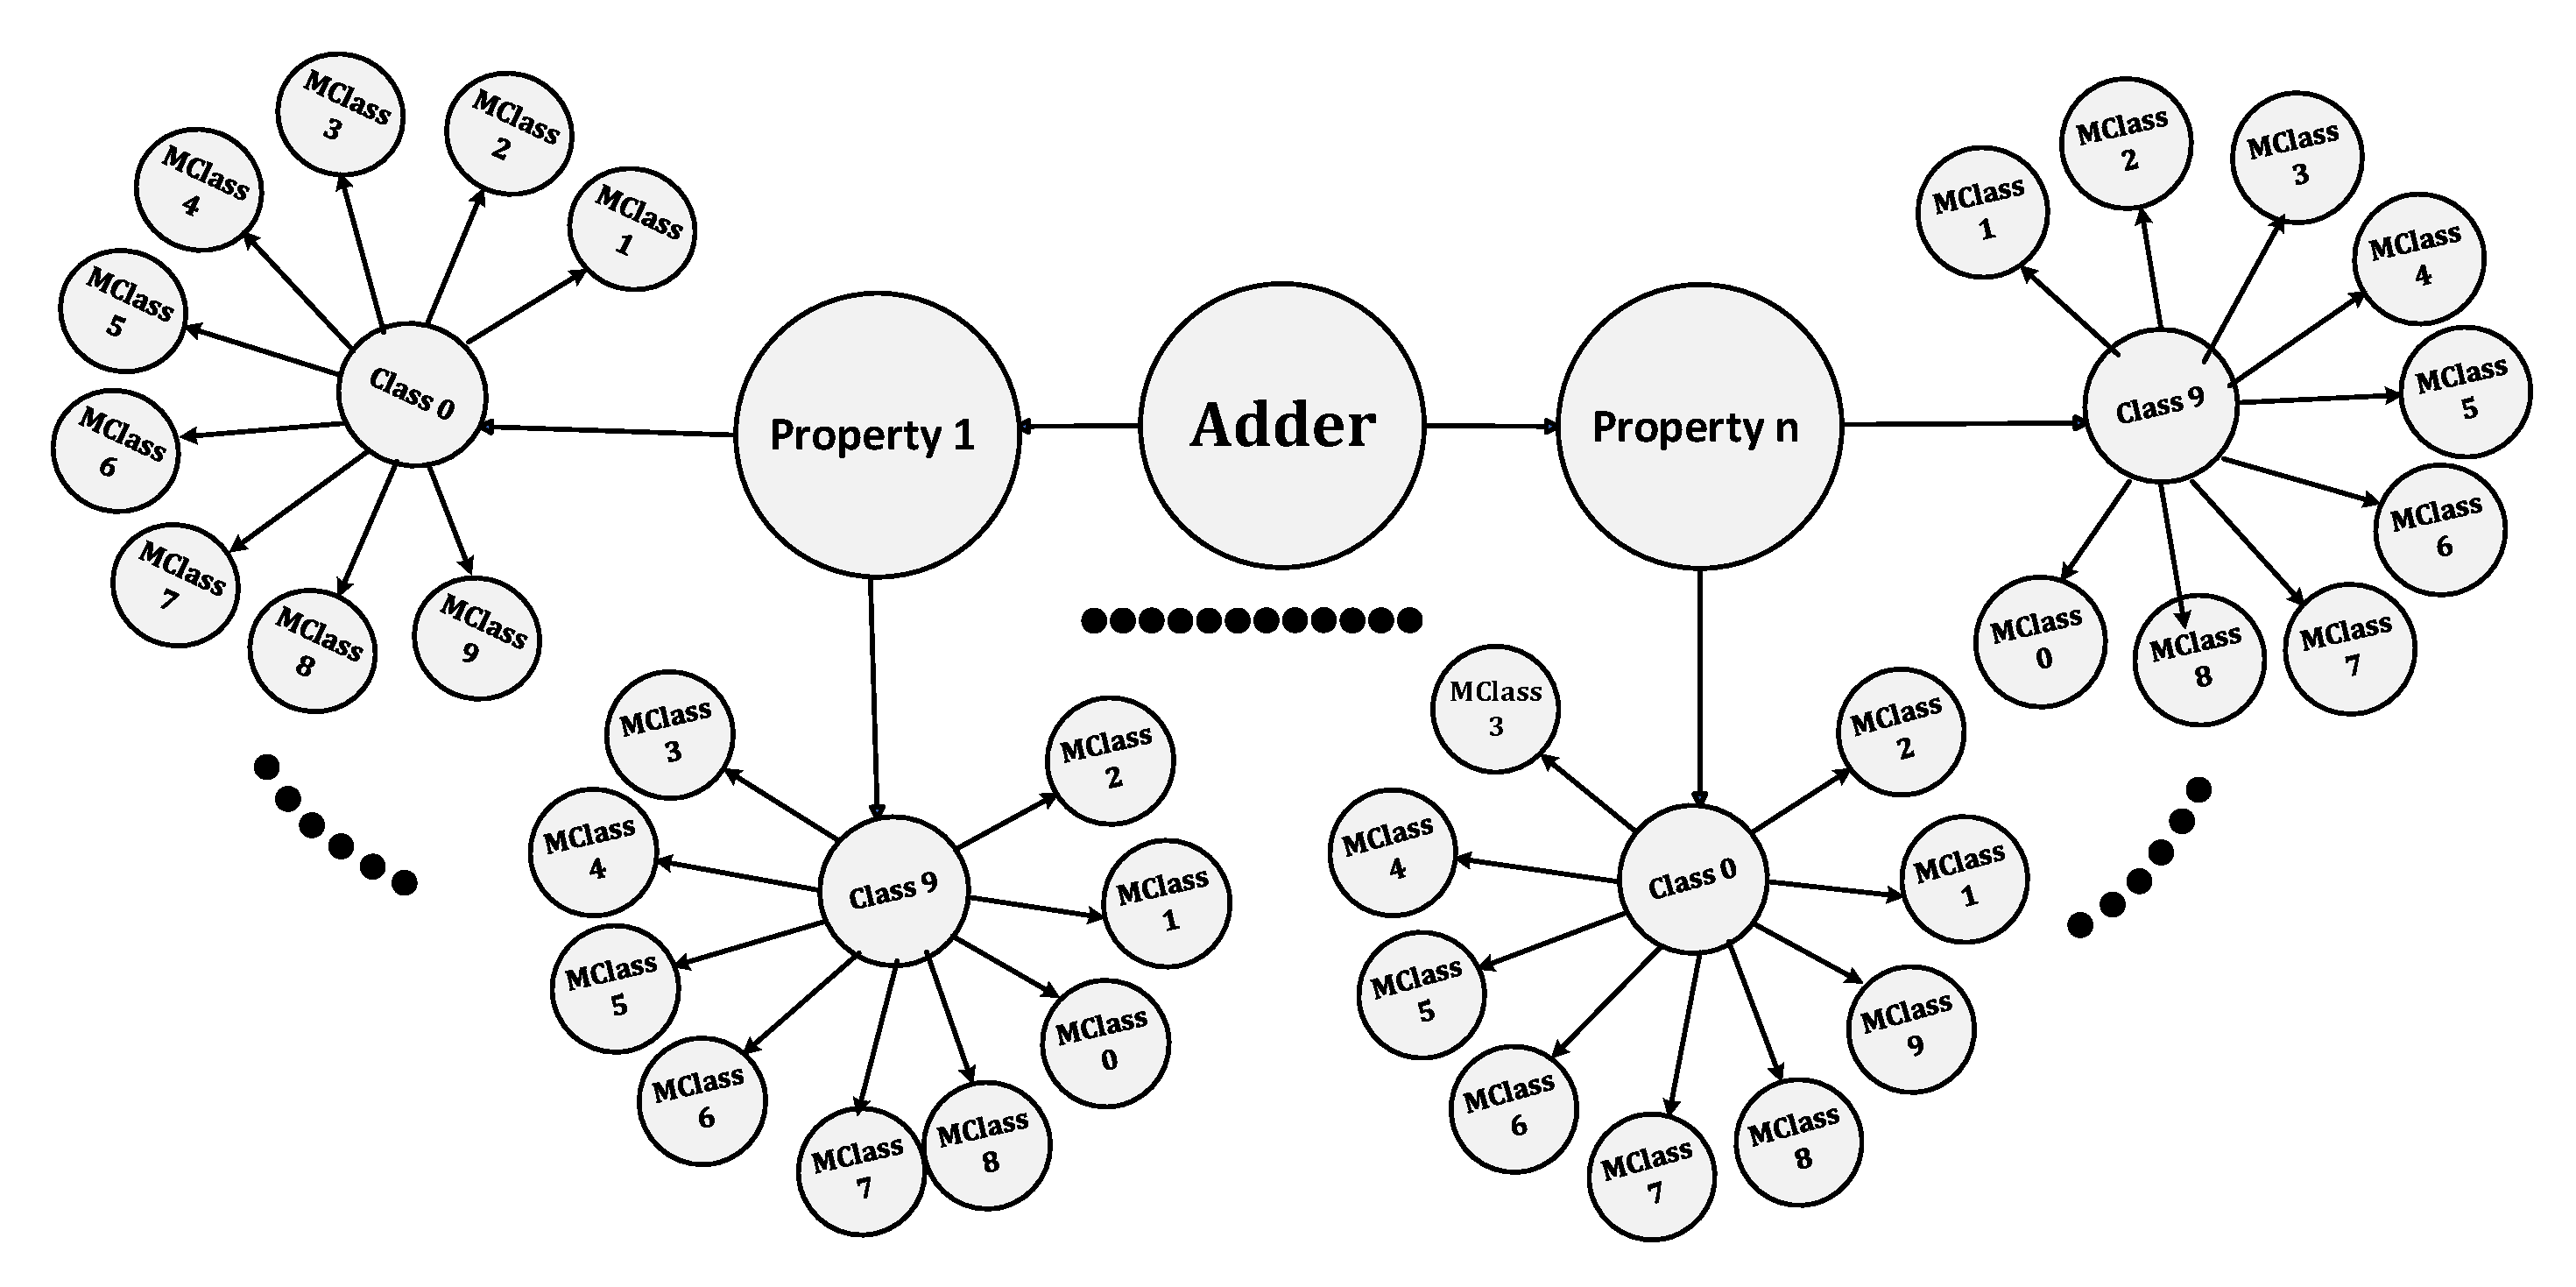
\includegraphics[width=\textwidth]{figures/step5.pdf}
    \caption{Error Summarization}
    \label{Summarization}
\end{figure*}



\section{Algorithm for Evaluating Model Robustness Using ProbLog}

\begin{algorithm}
  \caption{Evaluating Model Robustness Using ProbLog}
  \label{alg:model_robustness}
  \begin{algorithmic}[1]

  \REQUIRE $M$: Pre-trained model
  \REQUIRE $D$: Dataset
  \REQUIRE $N$: Number of samples per class
  \REQUIRE $P$: Set of properties

  \ENSURE $G$: Global correctness values for each specification

  \STATE \textbf{Load and Preprocess Data}
  \STATE $(X_{\text{train}}, y_{\text{train}}), (X_{\text{test}}, y_{\text{test}}) \leftarrow \text{load\_data}(D)$
  \STATE $X_{\text{test}} \leftarrow \text{preprocess\_data}(X_{\text{test}})$
  \STATE $\hat{Y} \leftarrow M.\text{predict}(X_{\text{test}})$
  \STATE $\hat{y} \leftarrow \text{extract\_predictions}(\hat{Y})$

  \STATE \textbf{Determine Number of Classes}
  \STATE $C \leftarrow \text{num\_classes}(y_{\text{test}})$ \COMMENT{Number of unique classes in the dataset}

  \STATE \textbf{Select Correctly Classified Samples}
  \STATE $\text{correct\_samples} \leftarrow \{ \}$
  \FOR{$c = 0$ \TO $C-1$} 
      \STATE $\text{correct\_samples}[c] \leftarrow \text{select\_correct\_samples}(X_{\text{test}}, y_{\text{test}}, \hat{y}, c, N)$
  \ENDFOR

  \STATE \textbf{Define Transformation Functions}
  \STATE $\text{define\_transformations}()$

  \STATE \textbf{Generate Test Cases}
  \FOR{$c = 0$ \TO $C-1$}
      \FORALL{$x \in \text{correct\_samples}[c]$}
          \FORALL{$T \in P$}
              \STATE $\text{generate\_test\_cases}(x, T)$
          \ENDFOR
      \ENDFOR
  \ENDFOR

  \STATE \textbf{Evaluate Model on Transformations}
  \FOR{$c = 0$ \TO $C-1$}
      \FORALL{$\text{property} \in P$}
          \STATE $L_{c, \text{property}} \leftarrow \text{compute\_accuracy}(M, \text{property}, c)$
      \ENDFOR
  \ENDFOR

  \STATE \textbf{Specification Definitions:}
  \STATE Specification1: $P(\text{Property1} \cap \text{Property2}) = P(\text{Property1}) \times P(\text{Property2})$ \COMMENT{AND relationship}
  \STATE Specification2: $P(\text{Property1} \cup \text{Property2}) = P(\text{Property1}) + P(\text{Property2}) - P(\text{Property1} \cap \text{Property2})$ \COMMENT{OR relationship}
  \STATE Specification3: Custom definitions
  \STATE \ldots

  \STATE \textbf{Generate and Evaluate ProbLog Code for Each Specification}
  \STATE Initialize $G$ as an empty list

  \FOR{$\text{spec} = 1$ \TO $\text{num\_specs}$}
      \STATE $\text{ProbLog Code}_{\text{spec}} \leftarrow \text{generate\_problog\_code}(L_{c, \text{property}}, \text{spec})$
      \STATE $G_{\text{spec}} \leftarrow \text{evaluate\_problog}(\text{ProbLog Code}_{\text{spec}})$
      \STATE Append $G_{\text{spec}}$ to $G$
  \ENDFOR

  \RETURN $G$
  \end{algorithmic}
\end{algorithm}

